% --------------------------------------------------------------
%                         Template
% --------------------------------------------------------------

\documentclass[10pt]{article} %draft = show box warnings
\usepackage[a4paper, total={6.5in,10.2in}]{geometry} % Flexible and complete interface to document dimensions
\usepackage[utf8]{inputenc} % Accept different input encodings [utf8]
\usepackage[T1]{fontenc}    % Standard package for selecting font encodings
\usepackage{lmodern} % Good looking T1 font\usepackage{tikz}
\usepackage{gensymb}


% --------------------------------------------------------------
%                       Packages
% --------------------------------------------------------------
\usepackage{float} % Improved interface for floating objects
\usepackage{amsmath,amsthm,amssymb} % American Mathematics Society facilities
\usepackage[linktoc=all]{hyperref} % create hyperlinks
\usepackage{graphicx,booktabs,array}
\usepackage{subcaption}
\usepackage{xcolor}
\usepackage{tikz}
\usepackage{algorithmicx}
\usepackage{algorithm}
\usepackage{algpseudocode}
\usepackage[framemethod=TikZ]{mdframed}
\usepackage{epstopdf}
% --------------------------------------------------------------
%                       Exercise Env
% --------------------------------------------------------------

\newtheoremstyle{question-style}% name of the style to be used
  {20pt}% measure of space to leave above the theorem. E.g.: 3pt
  {3pt}% measure of space to leave below the theorem. E.g.: 3pt
  {}% name of font to use in the body of the theorem
  {}% measure of space to indent
  {}% name of head font
  {}% punctuation between head and body
  { }% space after theorem head; " " = normal interword space
  {\bfseries Question \thmnumber{#2}.}% Manually specify head
  
\theoremstyle{question-style}
\newtheorem{answer}{\arabic{answer}}

% --------------------------------------------------------------
%                       Document
% --------------------------------------------------------------
\begin{document}
\date{August 2018}
% --------------------------------------------------------------
%                       Header
% --------------------------------------------------------------
\noindent
\normalsize\textbf{Reconnaissance des formes pour l’analyse et l’interprétation d’images} \hfill \textbf{Sorbonne Université}\\
\normalsize\textbf{RDFIA} \hfill \textbf{October 2019}
\flushright{\small Roger Leite Lucena -- \texttt{rogerleitelucena@gmail.com} }

{\small Alexandre Ribeiro João Macedo --  \texttt{arj.macedo@gmail.com}}\vspace{20pt}

\begin{flushleft}


\section*{TD 1,2 - SIFT and BoW}

\begin{answer} % Questão 1
\begin{align*}
    h_y = \frac{1}{2} \begin{bmatrix}
    1 \\
    2 \\
    1
    \end{bmatrix} 
    \qquad
     h_x = \frac{1}{2} \begin{bmatrix}
    -1 \\
    0 \\
    1
    \end{bmatrix}
\end{align*}

\begin{align*}
    M_x = h_y \times h_x^T = \frac{1}{4} \begin{bmatrix}
    -1 & 0 & 1\\
    -2 & 0 & 2 \\
    -1 & 0 & 1
    \end{bmatrix}
    \qquad
    M_y = h_x \times h_y^T = \frac{1}{4} \begin{bmatrix}
    -1 & -2 & -1 \\
    0 & 0 & 0 \\
    1 & 2 & 1
    \end{bmatrix}
\end{align*}
\end{answer}

\begin{answer}
By separating the convolution filter, we reduce the computational cost of the operation. Instead of running one convolution with 9 multiplications we run two convolutions with 3 multiplications each for a total of 6 multiplications.
\end{answer}

\begin{answer}
We use the gaussian mask to add a bigger weight to the points in the center of pad in which we are calculating the gradient.
\end{answer}

\begin{answer}
The discretization of orientations is useful to make it possible for the 4x4 regions of the patch to be assignable to an array of dimension 8 (result of a voting process for each gradient direction by the pixels of that region - it is equivalent to a histogram of the distribution of the different directions). Thus, it allows the creation of a signature of the patch by concatenating the signatures of each of its regions. \\

\quad Using more than $8$ directions (discretization of the directions over every $45\degree$) for the voting process mentioned above, using $360$ directions (one for every $1\degree$), for example, could work but it would also add noise to the system. Meaning that if you have too many candidates (using the voting analogy), it is likely in this context that each point in the gradient could vote for a different direction than the one it is indeed from (if they are so finely grained). \\ 

\quad In addition to that, this discretization in $8$ directions makes the algorithm more robust to rotation, since minor rotations would not change significantly the buckets of the voting process given that we have a margin of $45\degree$ for each bucket.

\quad Also, the arrays representing each region of the patch would be of size 360 now (instead of 8 - since it would be required 360 “buckets” for the “voting process”), globally requiring 45 times more memory than before and also making it computationally more expensive to calculate distances/similarities between SIFTs.
\end{answer}

\begin{answer}
We post process the SIFTs in order to remove noises. That means that only values above certain value will be returned normalized in the final calculations.
\end{answer}

\begin{answer} % Question 6
The SIFT is a reasonable way to describe numerically an image patch for image analysis because it is able to identify the local features in said image and assign it to a 128-array in a robust and reproducible way. This happens because the signature is calculated from the properties of the image that are robust to common manipulations.

\quad When we say common manipulations we mean mainly rotation (since an orientation is calculated for each keypoint, and further calculations are done relative to this orientation) and scaling (since a scale space is generated) - more details \href{http://aishack.in/tutorials/sift-scale-invariant-feature-transform-introduction/}{\color{blue}\underline{here}}. It is also robust to changes in the point of view (under a certain limit that depends on the way it was implemented) and to changes in the level of brightness (before the saturation point). These are some of the reasons why SIFT can be a reasonable way of numerically describing an image patch for image analysis. 
\end{answer}

\begin{answer}

First, we shall analyze the image representing the gradients in the two orthogonal directions:

\begin{figure}[H]
	\begin{center}
		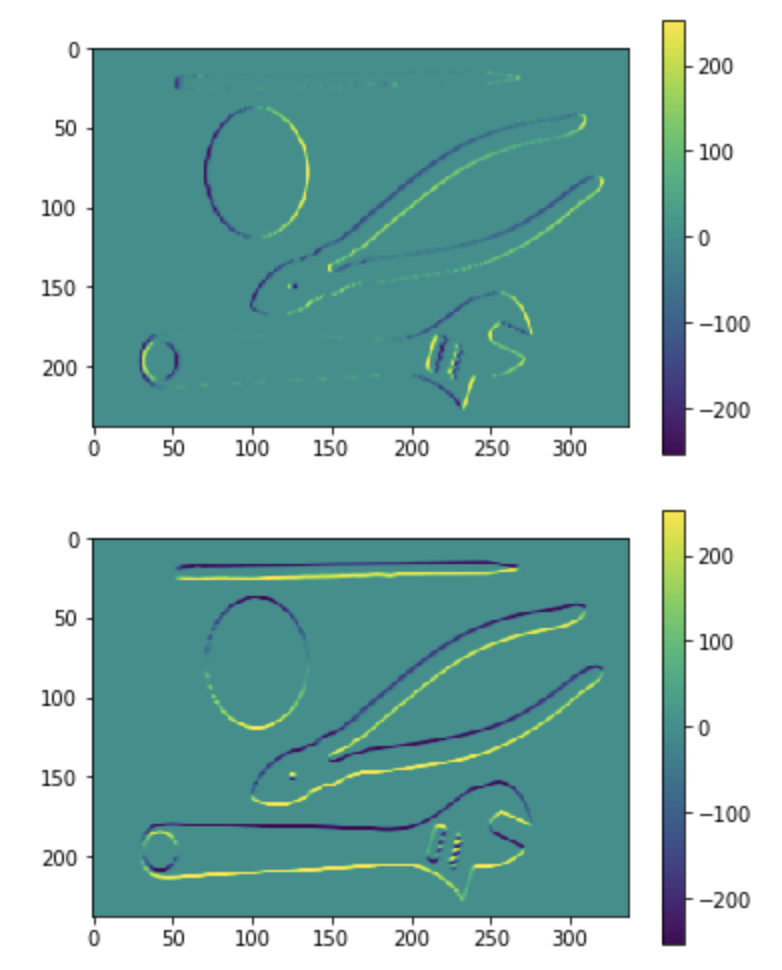
\includegraphics[scale=0.6]{gradients.png}
	\end{center}
	\caption{Gradient matrices - first with respect to "x" and then "y"}
	\label{fig:gradients}
\end{figure}

\quad The gradient matrices above are good to highlight the borders in the image, since these are the places on which we have the most variance. It is interesting how, indeed, the matrix gradient with respect to "x" is "blind" when we have variations only in the vertical "y" axis of the image - look at how the borders of the first and fourth tools in the first image are not well defined, compared to the second image. 

\quad To interpret the other results we can take the following example, to illustrate:  

\begin{figure}[H]
	\begin{center}
		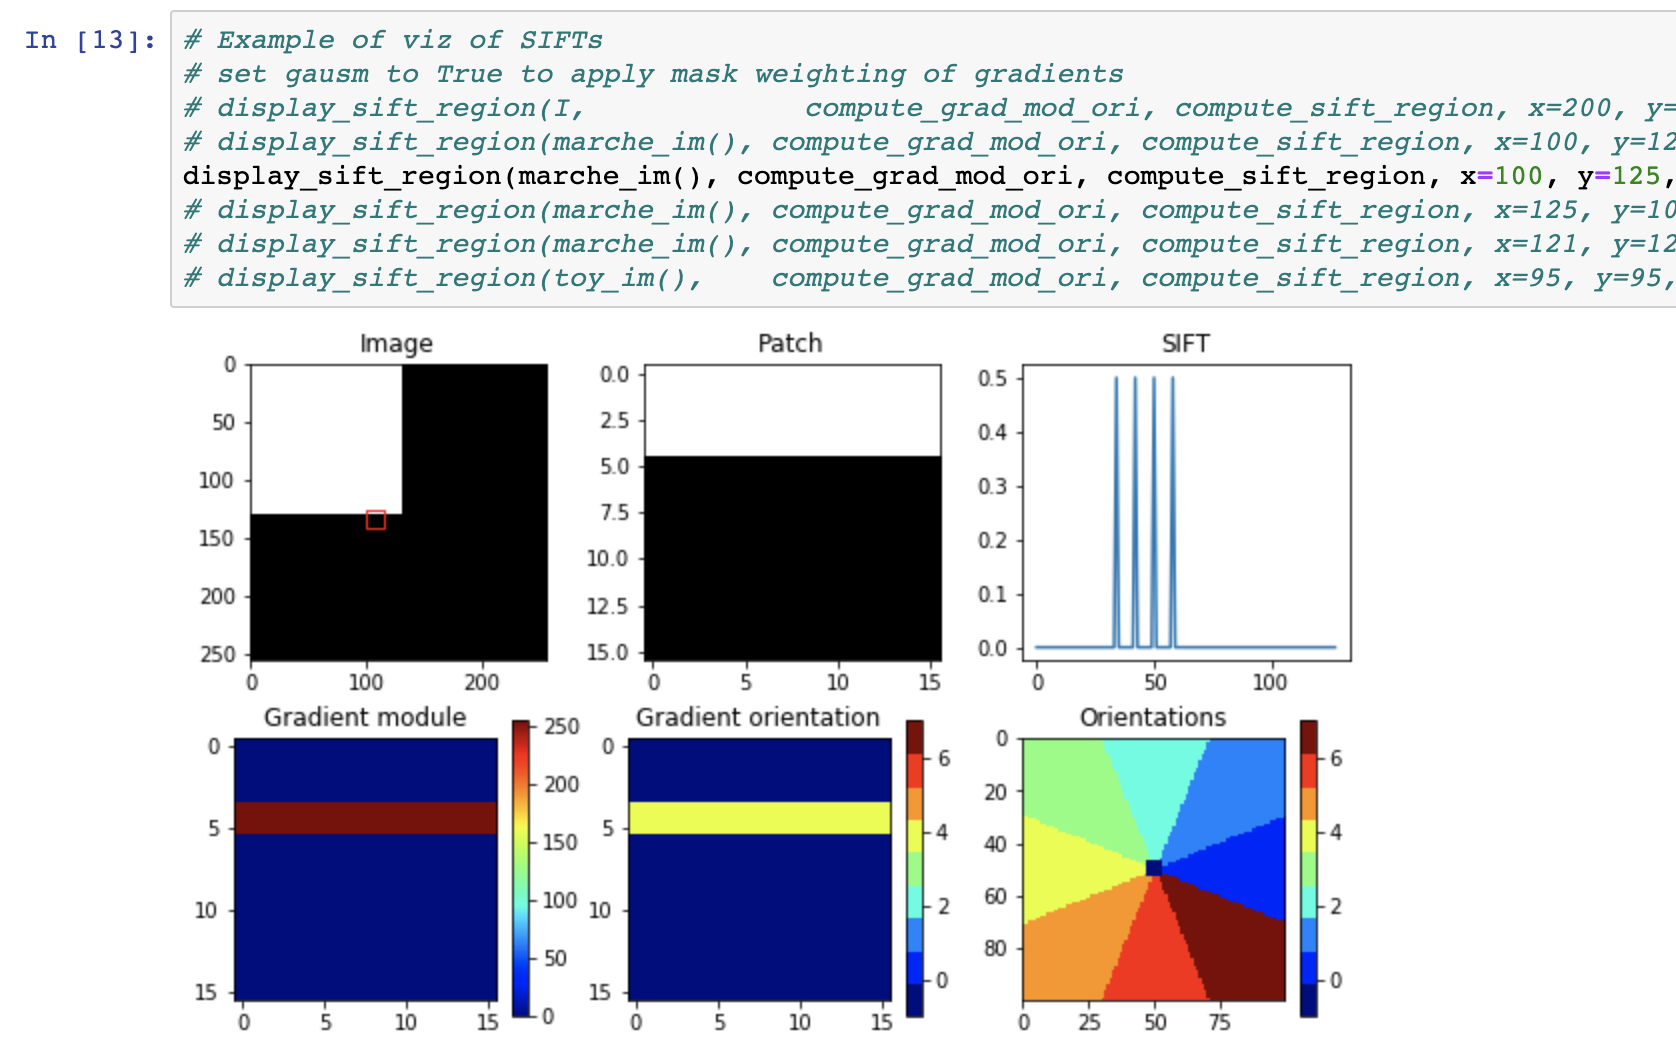
\includegraphics[scale=0.5]{regions.png} %[width=18cm, height=19cm]
	\end{center}
	\caption{Analysis of a SIFT - descriptor of a given patch}
	\label{fig:regions}
\end{figure}

\quad Knowing that the patch is divided in 16 regions (4x4), we can see that for the first four regions (first "row") there is no gradient in any direction, that is why the graph entitled SIFT is kept at zero during this first moment. Then, for the following 4 regions (second "row" of the patch), we have that the gradient is not zero anymore, it has the same non-zero value for the four of the regions - that is why we have fours consecutive peeks of the same height in the graph. After that, for the following $8$ regions of the patch (bottom half of the patch) we are again in regions with no gradient at all in any direction, resulting in a graph kept in zero once again.

\end{answer}

\begin{answer} % Question 8
It is important for the reason that it creates a global way of describing the images and comparing them one with the others. 

\quad Namely: before, every image had their own SIFTs. Now, with the dictionary, we can represent every image using the same visual words (representing each image by the same "histogram"-like vector whose dimension is the size of the dictionary), allowing us to compare them properly.

\end{answer}

\begin{answer}
\begin{align*}
    f(c) = \sum_i \Vert x_i -c \Vert_2^2 \\
    \nabla f = \sum_i 2 (x_i -c) \\
    \nabla f = 0 \implies n c = \sum_i x_i \\
    c = \frac{1}{n} \sum_i x_i
\end{align*}
\end{answer}

\begin{answer} % Question 10
We shall use the "Elbow method": first, for every number "k" of clusters, we plot in a graph the total intra-cluster variation (or Within-cluster Sum of Square - WSS). This WSS measures the compactness of the clustering, and we want it indeed to be as small as possible. Then, we choose a number "k" of clusters so that adding another cluster does not improve a lot the total WSS - the "elbow" or "knee" in the plot.

\end{answer}

\begin{answer}
This way we can see the concrete examples of patches related to each visual word - these patches are representations of the meaning behind every visual word in the dictionary since these words themselves do not necessarily represent a meaningful image (they are the mathematical vector results of the k-means algorithm, namely: the cluster centers).
\end{answer}

\begin{answer} % Question 12
We managed in our notebook to, in a first moment with only 6 clusters (the $6^{th}$ being the "zero-vector cluster"), indeed visualize the $9$ resembling closest patches to every cluster center - a confirmation that they are indeed similar and a presentation of a common pattern underlying that cluster.

\begin{figure}[H]
	\begin{center}
		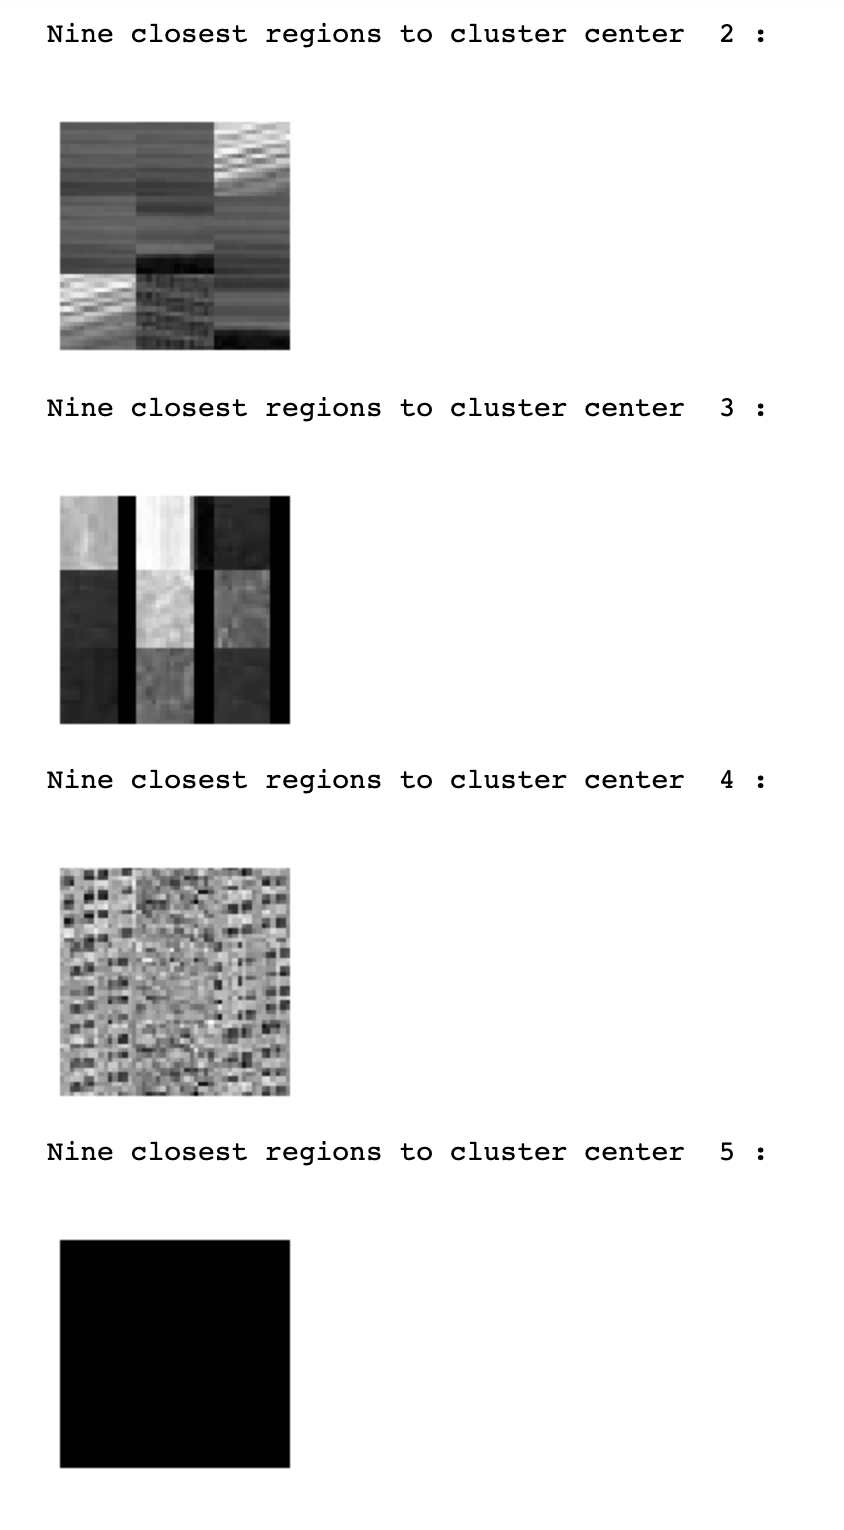
\includegraphics[scale=0.6]{clusters.png} %[width=18cm, height=19cm]
	\end{center}
	\caption{Nine closest patches to some cluster centers}
	\label{fig:clusters}
\end{figure}

\quad Also, looking at the $6^{th}$ cluster, we have as expected all-black patches - the ones that should indeed be around the $0$-vector cluster center. 
\end{answer}

\begin{answer} 
It represents a "histogram"-like vector that was normalized, on which the votes are given to each visual word in the dictionary (a position of $z$) if we had SIFTs on that image that were clustered around that visual word (cluster center). \\

\quad That is, $z$ can be understood as a signature of the image made from how frequent some visual words are present in it - every visual word represented by a position in $z$ with a given relative weight assigned.
\end{answer}

\begin{answer} % Question 14

For $6$ clusters we have the following final result:

\begin{figure}[H]
	\begin{center}
		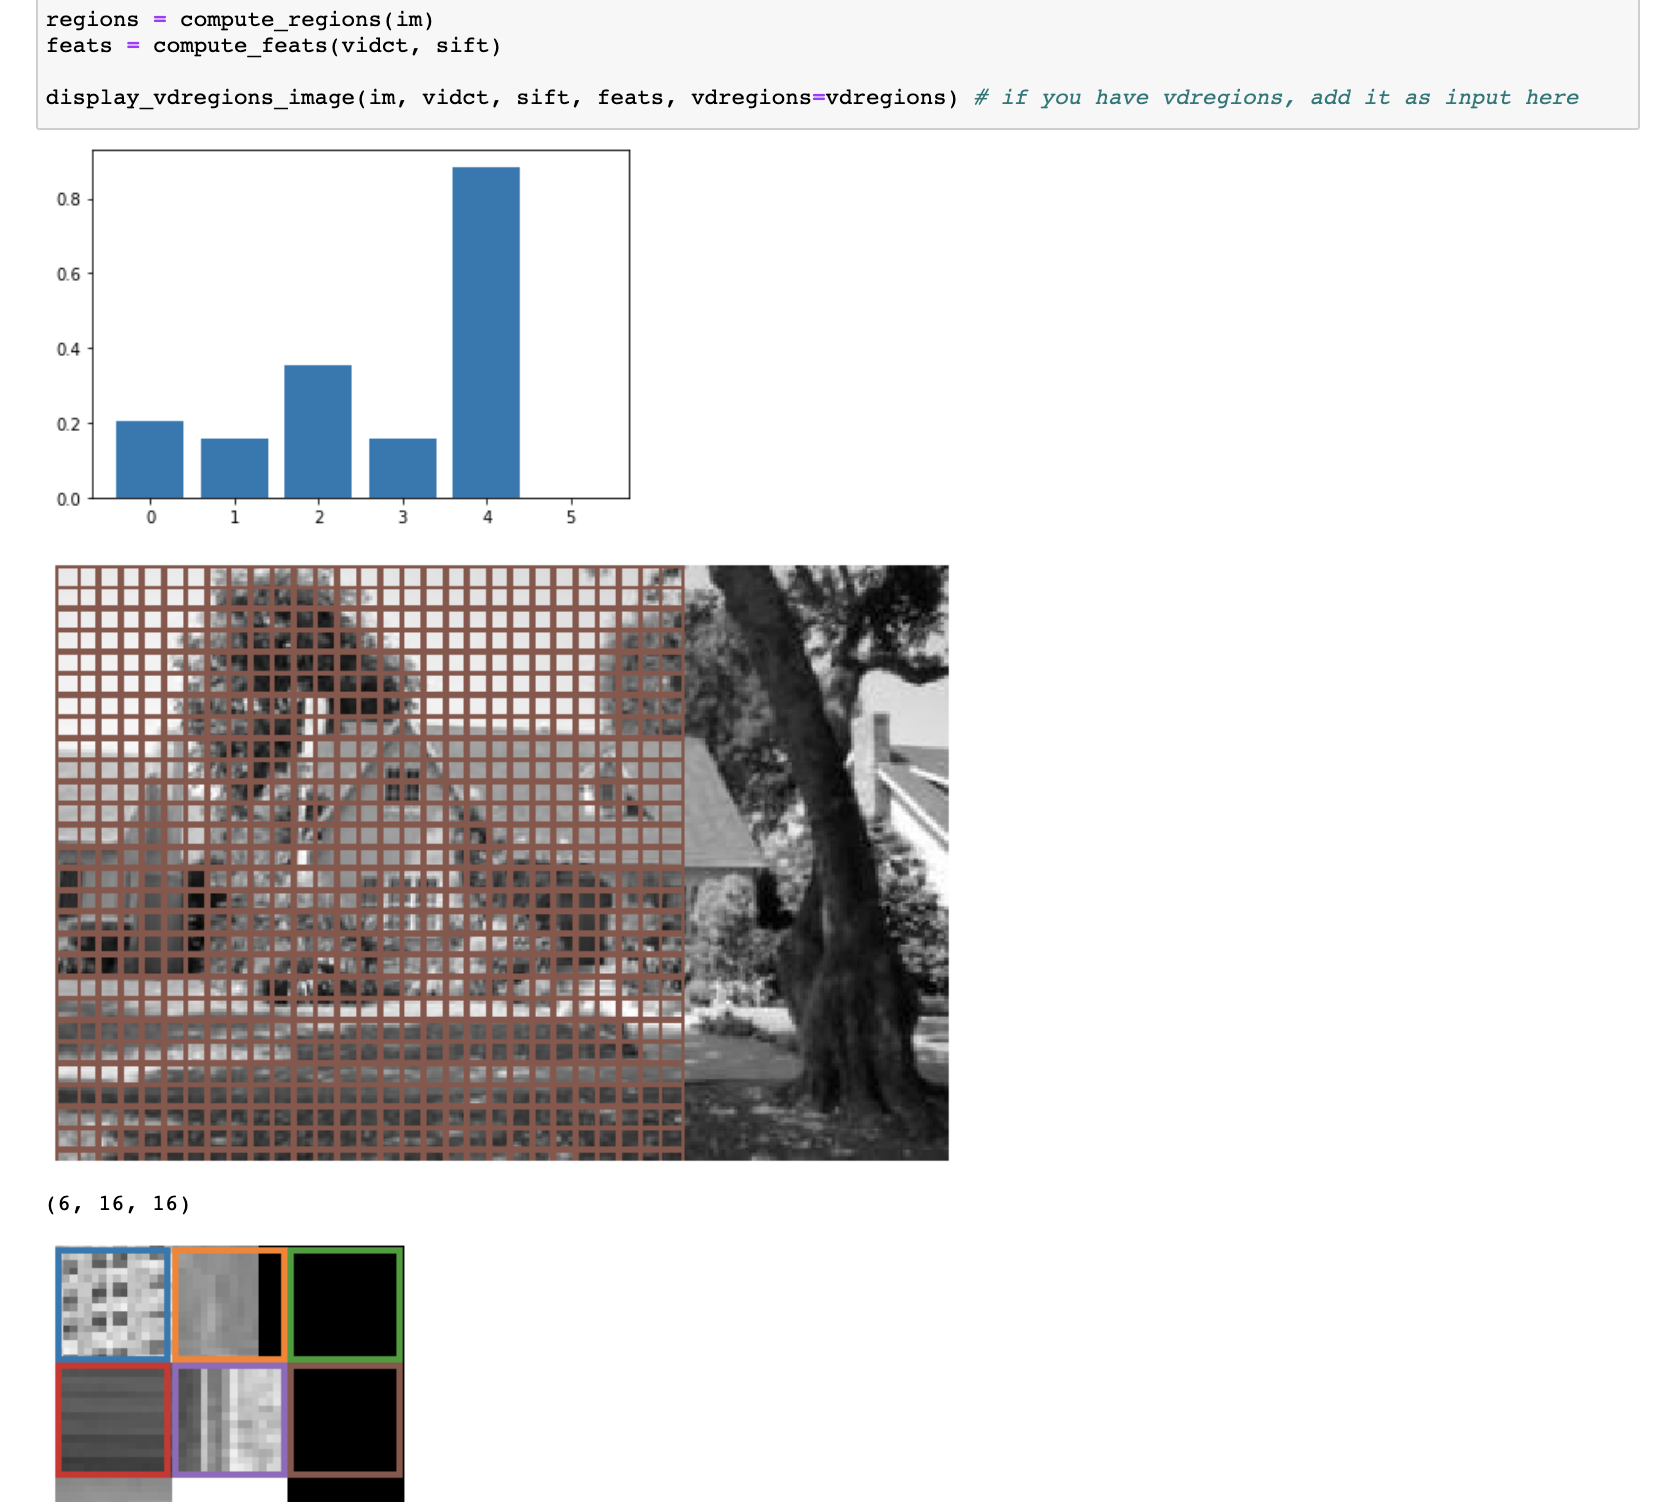
\includegraphics[scale=0.6]{final.png} %[width=18cm, height=19cm]
	\end{center}
	\caption{Representation of the "histogram"-like "z" vector using 6 clusters followed by some representative patches of the clusters}
	\label{fig:final}
\end{figure}

\quad Analyzing it, take the cluster number $4$, for example, the one with the highest peek in "z" above. When going through the \textbf{question 12} we saw that this cluster is represented by a kind of textured pattern, like a noised grid. Looking at the image we can see that it is indeed supposed to be present in a number of regions, like in the grass, the leaves and the walls of the house for example. So, it is reasonable that we had a peek for this cluster in the image above.

\end{answer}

\begin{answer}
Using "nearest neighbor" is interesting because this way we are affecting, to each SIFT, only one visual word (the one that is the most similar and then tend to be the most representative of it), simplifying the "coding" step. \\

\quad We could also use some other "codings" such as: "to each descriptor associate the two nearest visual words" or "the three nearest visual words, with different weights (based on the inverse of the distance to that words)", or variations of that.
\end{answer}

\begin{answer} % Question 16
The "sum pooling" is interesting because it makes the system corresponds to a voting process on which every descriptor SIFT votes to a visual word, simplifying the pooling step, with a normalization for "z" being done by the end. \\

If we had used the inverse of the distances for the "coding" step, for example, we could use a "max" pooling, or sum the two "max" for every visual word, and so on. 

\end{answer}

\begin{answer}
This normalization is important because now, independently of the number of votes (that can be different from one image to the other depending on the way the patches and the SIFTs were taken from it in the first place), the final "z" vectors representing each image become comparable to one another - like vectors in the same normalized space. For this, the $L_2$ norm fits like a glove. \\

We could use other norms too, obtaining similar histograms for "z" as in the \textbf{question 14}.
\end{answer}

\setcounter{answer}{0}
\section*{TD 3 - SVM}
\begin{answer} % Questão 1
For the value of C that gave the best score in the validation test we get a score of 0.559 over the test set.
\begin{figure}[htbp]
	\centering
	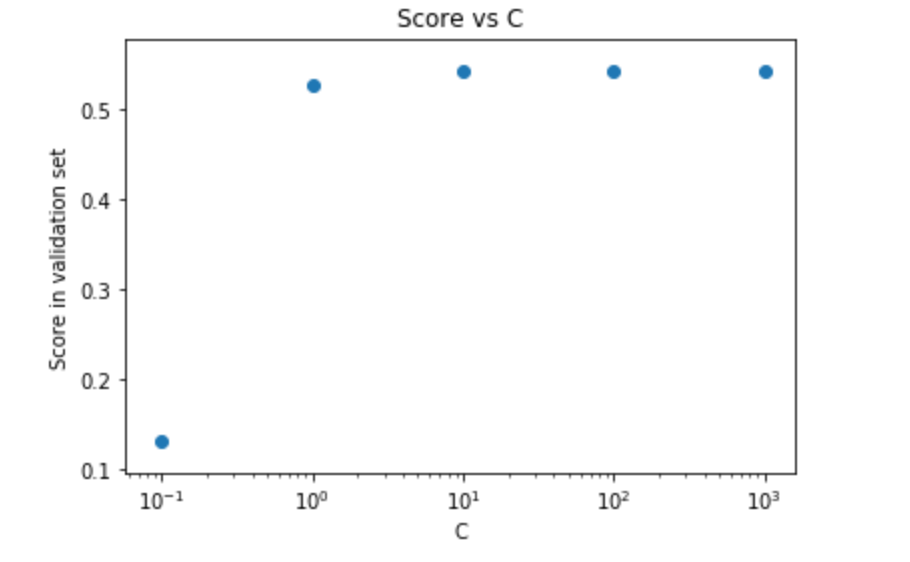
\includegraphics[width=0.5\columnwidth]{d.png}
	\caption{Score for different values of C}
\end{figure}
\end{answer}
\begin{answer}
The validation set is needed alongside the test set so we can find a value of C that gives the best score and by using a different set for validation and testing we avoid choosing a C that has some bias towards the data used to do the testing.
\end{answer}
\begin{answer}
A possible processing pipeline for a gray scale image in order to classify it is to calculate the SIFT using the pipeline used in TMEs 1-2. Once we have the SIFTs for the image, we can compute its features and finally, we can use the pre-trained SVM to predict the labels of the image.
\end{answer}
\begin{answer}
One way to improve the processing, specially in the feature extraction part is to parallelize the computations. The code used in the TME is using a single core to make all calculations. This is suboptimal and does not profit from the current hardware advancements.
\end{answer}

\end{flushleft}
\end{document}
